\section{Алгебра логики} \label{sec:boolean}

\defemph{Математика}~--- это общий язык для многих сфер деятельности человека, позволяющий формализовать объекты, которыми оперирует наш разум.
Однним из важнейших разделов математики считается \defemph{математическая логика},
так как именно она является фундаментом математических суждений, исследует природу математического доказательства в целом.
Поэтому не зря курс дискретного анализа начинается именно с \defemph{алгебры логики}~---
объекта математической логики, хоть и сравнительно простого, но важного и полезного.



\subsection{Булева алгебра}
\label{subsec:boolean:algebra}


Алгебра логики изучает логические операции над высказываниями.
При этом в простейшем случае считается, что высказывания могут быть только истинными (обозначается~<<$ 1 $>>) или ложными (обозначается~<<$ 0 $>>);
%такие высказывания являются \defemph{булевозначными}.

\begin{definition}
    Переменные, принимающие значения только $ 0 $ или $ 1 $, называются \defemph{булевыми переменными}.
    Аналогично, функции от булевых переменных, принимающие только значения $ 0 $ или $ 1 $~--- \defemph{булевы функции}, или \defemph{логические операции}, \defemph{связки}.
    \defemph{Высказываниям} ставится в соответствие либо булева переменная с фиксированным значением, либо значение булевой функции на фиксированных аргументах.
\end{definition}

Примеры логических операций:
<<НЕ>> (обозначается~<<$ \neg $>>),
<<И>> (обозначается~<<$ \wedge $>>),
<<ИЛИ>> (обозначается <<$ \vee $>>),
исключающее <<ИЛИ>> (обозначается <<$ \oplus $>>),
импликация (обозначается <<$ \rightarrow $>>),
эквивалентность (обозначается <<$ \leftrightarrow $>>).

Заметим, что как и любые другие функции с конечной областью определения, булевы функции можно задать таблицей, просто перечислив их значения на всех возможных значениях аргументов.
Данные таблицы называются \defemph{таблицами истинности}.

\begin{table}[ht!]
    \center
    \begin{tabular}{|c|c|c|c|c|c|c|c|}
         \hline
         $ A $  &  $ B $  &  $ \neg A $  &  $ A \wedge B $  &  $ A \vee B $  &  $ A \oplus B $  &  $ A \rightarrow B $  &  $ A \leftrightarrow B $ \\
         \hline
         \hline
         $ 0 $  &  $ 0 $  &  $ 1 $       &  $ 0 $           &  $ 0 $         &  $ 0 $           &  $ 1 $                &  $ 1 $                   \\
         $ 0 $  &  $ 1 $  &  $ 1 $       &  $ 0 $           &  $ 1 $         &  $ 1 $           &  $ 1 $                &  $ 0 $                   \\
         $ 1 $  &  $ 0 $  &  $ 0 $       &  $ 0 $           &  $ 1 $         &  $ 1 $           &  $ 0 $                &  $ 0 $                   \\
         $ 1 $  &  $ 1 $  &  $ 0 $       &  $ 1 $           &  $ 1 $         &  $ 0 $           &  $ 1 $                &  $ 1 $                   \\
         \hline
    \end{tabular}
    \caption{задание логических связок таблицами истинности}
    \label{tab:boolean:truth_tables}
\end{table}

%\begin{Exercise}[counter=SecExercise, title=(КЗ №1)]
%    \noindent
%    Для какого слова \textbf{ложно} высказывание <<Первая буква слова гласная $ \rightarrow $ (Вторая буква слова гласная $ \vee $ Последняя буква слова гласная)>>?
%    \begin{enumerate}[label=\arabic*)]
%        \item жара;
%        \inlineitem орда;
%        \inlineitem огород;
%        \inlineitem парад;
%    \end{enumerate}
%\end{Exercise}
%
%\begin{Answer}
%    \noindent
%    Подставляя слова в элементарные высказывания, получаем
%    \begin{enumerate}
%        \item $ 0 \rightarrow (1 \vee 1) = 1 $;
%        \item $ 1 \rightarrow (0 \vee 1) = 1 $;
%        \item $ 1 \rightarrow (0 \vee 0) = 0 $;
%        \item $ 0 \rightarrow (1 \vee 0) = 1 $;
%    \end{enumerate}
%    Можно было сразу отсеять первый и четвёртый варинат по ложной посылке, а ответ найти по ложному следствию.
%\end{Answer}

%\shipoutAnswer

Запись таблицы истинности можно сократить, если изначально условиться, в каком порядке перечисляются возможные значения аргументов, и оставить только столбец значений функции;
этот столбец тогда будет являться \defemph{булевым вектором} (\defemph{вектором значений}), задающим функцию.
Стандартный порядок перечисления значений аргументов таков, чтобы они образовывали двоичную запись номера строки (см. таблицу \ref{tab:boolean:truth_tables}).

\begin{example}
    Операция <<НЕ>> задаётся булевым вектором $ 10 $, а, например, импликация~--- $ 1101 $.
\end{example}

Булевы функции можно также задавать при помощи формул, <<собирая>> из других связок.
Фообще говоря, формула является деревом, задающим порядок применения составляющих формулу связок к аргументам и к значениям других связок.
Однако такой взгляд на вещи полностью эквивалентен стандартному написанию математических формул, если задать приоритет операций, или просто использовать скобки.
Приоритет изученных связок указан в таблице \ref{tab:boolean:full_info}, пример формулы и соответствующего ей дерева~--- на рис. \ref{fig:boolean:tree_example}.

\begin{table}[ht!]
    \center
    \begin{tabular}{|c|c|c|c|c|c|}
        \hline
        Связка               & Приоритет & \makecell{Краткое \\ название}     & Название        & Смысл                       \\
        \hline
        \hline
        $ \neg $             & $ 1 $     & <<НЕ>>                             & отрицание       & <<не $ A $>>                \\
        $ \wedge $           & $ 2 $     & <<И>>                              & конъюнкция      & <<$ A $ и $ B $>>           \\
        $ \vee $             & $ 3 $     & <<ИЛИ>>                            & дизъюнкиця      & <<$ A $ или $ B $>>         \\
        $ \oplus $           & $ 3 $     & \makecell{<<ИСКЛИЛИ>>, \\ <<XOR>>} & исключающее или & <<либо $ A $, либо $ B $>>  \\
        $ \rightarrow $      & $ 4 $     & --                                 & импликация      & <<если $ A $, то $ B $>>    \\
        $ \leftrightarrow $  & $ 5 $     & --                                 & эквивалентность & <<$ A $ равносильно $ B $>> \\
        \hline
    \end{tabular}
    \caption{информация о логических связках}
    \label{tab:boolean:full_info}
\end{table}


\begin{figure}[ht!]
\center
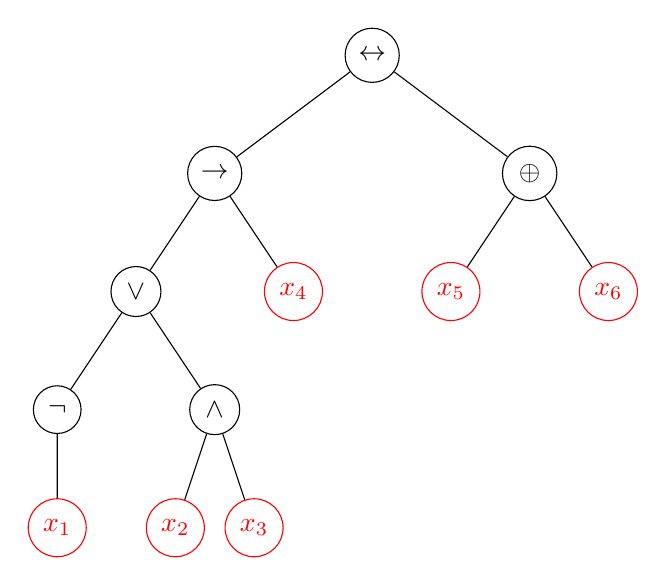
\begin{tikzpicture}[level distance=1.5cm,
    level 1/.style={sibling distance=4cm},
    level 2/.style={sibling distance=2cm},
    level 4/.style={sibling distance=1cm}
    %edge from parent/.style={draw, edge from parent path={(\tikzparentnode) -- (\tikzchildnode)}}
]
\tikzstyle{every node}=[circle,draw]

\node (Root) {$ \leftrightarrow $}
    child {
        node {$ \rightarrow $}
        child {
            node {$ \vee $}
            child {
                node {$ \neg $}
                child { node[red] { $x_1 $} }
            }
            child {
                node {$ \wedge $ }
                child { node[red] { $ x_2 $ } }
                child { node[red] { $ x_3 $ } }
            }
        }
        child { node[red] {$ x_4 $} }
    }
    child {
        node {$ \oplus $}
        child { node[red] {$ x_5 $} }
        child { node[red] {$ x_6 $} }
    };

\end{tikzpicture}
\caption{дерево формулы $ \neg x_1 \vee x_2 \wedge x_3 \rightarrow x_4 \leftrightarrow x_5 \oplus x_6 $
(или, что то же самое, $ (((\neg x_1) \vee (x_2 \wedge x_3)) \rightarrow x_4) \leftrightarrow (x_5 \oplus x_6) $)}
\label{fig:boolean:tree_example}
\end{figure}

\FloatBarrier



\subsection{Логические законы}
\label{subsec:boolean:laws}



\defemph{Логический закон} (\defemph{тождество})~--- равенство двух булевых функций, заданных разными формулами.
Равенство булевых функций определяется так же, как и равенство любых других функций:
требуется равенство областей определений функций и равенство значений функций в любой точке области определения.
Равенство формул и области определения, очевидно, влечет равенство функций; обратное не верно.
Принято также считать, что если аргументы в формуле пронумерованы, то число аргументов равно максимальному индексу (<<нет пропусков>>).

\begin{example}
    \label{example:boolean:formulas}
    \begin{itemize}
        \item[] % КОСТЫЛЬ! :(
        \item С точки зрения правил школьной математики, функции $ \sqrt[3]{x} $ и $ (x)^{1/3} $ не равны.
        \item Формула, задающая функцию трёх аргументов: $ x_1 \wedge x_3 $.
        \item Две формулы, задающие одну и ту же функцию: $ x_1 \rightarrow x_2 $ и $ \neg x_1 \vee x_2 $.
        \item Равенство областей определения \textbf{существенно}: пусть
            \[
                f(A,B,C) = A \vee B, \quad g(A,B) = A \vee B
            \]
            Данные две функции заданы одной и той же формулой, но $ f \neq g $.
    \end{itemize}
\end{example}

В случае булевых функций определение равенства можно записать иначе, если воспользоваться понятием \defemph{тавтологии}.

\begin{definition}
    Функция $ g $ называется \defemph{тавтологией} $ \defarr $ она тождественна равна единице на всей области определения.
\end{definition}

\begin{remark}
    Для булевых функций $ f $ и $ g $ их равенство эквивалентно равенству областей определений и тавтологичности $ f \leftrightarrow g $.
\end{remark}


Пользуясь определением связок из таблицы \ref{tab:boolean:truth_tables}, можно доказать множество логических законов. %(тождеств).
Самые тривиальные законы~--- \textit{коммутативность} и \textit{ассоциативность} операций $ \wedge $, $ \vee $ и $ \oplus $:
\[
    x_1 \wedge x_2 = x_2 \wedge x_1, \qquad
    x_1 \vee x_2   = x_2 \vee x_1, \qquad
    x_1 \oplus x_2 = x_2 \oplus x_1
\]
\[
    x_1 \wedge (x_2 \wedge x_3) = (x_1 \wedge x_2) \wedge x_3, \qquad
    x_1 \vee (x_2 \vee x_3)     = (x_1 \vee x_2) \vee x_3, \qquad
    x_1 \oplus (x_2 \oplus x_3) = (x_1 \oplus x_2) \oplus x_3
\]
Также имеет смысл выписать некоторые \textit{дистрибутивные} законы:
\[
    x_1 \wedge (x_2 \vee x_3) = (x_1 \wedge x_2) \vee (x_1 \wedge x_3)
\]
\[
    x_1 \vee (x_2 \wedge x_3) = (x_1 \vee x_2) \wedge (x_1 \vee x_3)
\]
Другие полезные законы:
\begin{enumerate}[label=\arabic*)]
    \item $ x_1 \vee (x_1 \wedge x_2) = x_1; \quad x_1 \wedge (x_1 \vee x_2) = x_1 $ \hspace*{\fill} \textit{(законы поглощения)}
    \item $ \neg (x_1 \wedge x_2) = \neg x_1 \vee \neg x_2; \quad \neg (x_1 \vee x_2) = \neg x_1 \wedge \neg x_2 $ \hspace*{\fill} \textit{(законы де Моргана)}
    \item $ x_1 \rightarrow x_2 = \neg x_2 \rightarrow \neg x_1 $ \hspace*{\fill} \textit{(закон контрапозиции)}
    %\item $ (x_1 \rightarrow x_2) \vee x_3 = x_1 \rightarrow (x_2 \vee x_3) $ \hspace*{\fill} \textit{(внос в следствие)}
    \item $ x_1 \leftrightarrow x_2 = \neg (x_1 \oplus x_2) = (x_1 \rightarrow x_2) \wedge (x_2 \rightarrow x_1) $
    \item $ x_1 \to x_2 = \neg x_1 \vee x_2 $ \label{item:implication_disjunction}
\end{enumerate}
Остальные законы и свойства можно найти в конспекте лекций Александра Александровича.
Отдельно отметим, что из пункта \ref{item:implication_disjunction} следует,
что импликация дистрибутивна относительно конъюнкции:
\[
    x_1 \rightarrow (x_2 \wedge x_3) = \neg x_1 \vee (x_2 \wedge x_3) = (\neg x_1 \vee x_2) \wedge (\neg x_1 \vee x_3) = (x_1 \rightarrow x_2) \wedge (x_1 \rightarrow x_3)
\]

\begin{Exercise}[counter=SecExercise, label={ex:boolean:chain}]
    \noindent
    Докажите равенство функций
    \[
        (x_1 \rightarrow x_2) \wedge (x_2 \rightarrow x_3) \wedge \ldots \wedge (x_{k-1} \rightarrow x_k) \wedge (x_k \rightarrow x_1) =
        \left( \bigwedge_{i=1}^{k-1} (x_i \rightarrow x_{i+1}) \right) \wedge (x_k \rightarrow x_1)
    \]
    и
    %\[
    %    (x_1 \leftrightarrow x_2) \wedge (x_2 \leftrightarrow x_3) \wedge \ldots \wedge (x_{k-1} \leftrightarrow x_k) \wedge (x_k \leftrightarrow x_1) =
    %    \left( \bigwedge_{i=1}^{k-1} (x_i \leftrightarrow x_{i+1}) \right) \wedge (x_k \leftrightarrow x_1)
    %\]
    \[
        x_1 \leftrightarrow x_2 \leftrightarrow x_3 \leftrightarrow \ldots \leftrightarrow x_k
    \]
\end{Exercise}

\begin{Answer}
    \noindent
    % Несложно заметить, что если $ \forall i, j \; x_i = x_j $, то оба высказывания истинны.
    % Если же $ \exists i,j: \; x_i \neq x_j $, то второе высказывание ложно.
    % Но что насчёт первого?
    % Понятно, что раз $ \exists i,j: \; x_i \neq x_j $, то и $ \exists m: \; x_m = 1 \neq 0 = x_{m+1} $
    % (считаем, что $ x_{k+1} = x_1 $, то есть нумерация зациклена).
    % Но тогда и первое высказывание ложно.
    %% ВЕРСИЯ БЕЗ КВАНТОРОВ %%
    Несложно заметить, что если при любых $ i, j $ выполнено $ x_i = x_j $, то оба высказывания истинны.
    Если же существуют $ i,j $ такие, что $ x_i \neq x_j $, то второе высказывание ложно.
    Но что насчёт первого?
    Понятно, что раз существуют $ i,j $ такие, что $ x_i \neq x_j $, то и существует $ m $ такое, что $ x_m = 1 \neq 0 = x_{m+1} $
    (считаем, что $ x_{k+1} = x_1 $, то есть нумерация зациклена).
    Но тогда и первое высказывание ложно.
\end{Answer}



\subsection{Преобразование и упрощение формул}
\label{subsec:boolean:transformation}



Преобразование формул при помощи одних тождеств позволяют находить другие.
Так при помощи привёдённых в предыдущем разделе законов можно доказать следующее утверждение:
\begin{statement}[Закон вноса в посылку и следствие]
    \label{statement:boolean:disjunction_implication}
    Верны тождества
    \[
        (x_1 \rightarrow x_2) \vee x_3 = x_1 \rightarrow (x_2 \vee x_3) = (x_1 \vee x_3) \rightarrow (x_2 \vee x_3)
    \]
\end{statement}

\begin{proof}
    Первое равенство доказывается тривиально:
    \[
        (x_1 \rightarrow x_2) \vee x_3 = \neg x_1 \vee x_2 \vee x_3 = \neg x_1 \vee (x_2 \vee x_3) = x_1 \rightarrow (x_2 \vee x_3)
    \]
    Перейдём ко второму.
    Для этого распишем импликацию через дизъюнкцию и воспользуемся правилом де Моргана:
    \[
        (x_1 \vee x_3) \rightarrow (x_2 \vee x_3) =
        \neg (x_1 \vee x_3) \vee x_2 \vee x_3 =
        (\neg x_1 \wedge \neg x_3) \vee x_2 \vee x_3
    \]
    Воспользовавшись дистрибутивностью дизъюнкции относительно конъюнкции, получаем
    \begin{multline*}
        (\neg x_1 \wedge \neg x_3) \vee x_2 \vee x_3 =
        \left[ (\neg x_1 \vee x_3) \wedge (\neg x_3 \vee x_3) \right] \vee x_2 = \\ =
        \left[ (\neg x_1 \vee x_3) \wedge 1 \right] \vee x_2 =
        \neg x_1 \vee x_3 \vee x_2 =
        x_1 \rightarrow (x_2 \vee x_3)
    \end{multline*}
\end{proof}

%При помощи доказанного факта решим следующую задачу:
\begin{Exercise}[counter=SecExercise, label={ex:boolean:disjunction_distributivity_over_equivalence}]
    \noindent
    Докажите дистрибутивность дизъюнкции относительно эквивалентности:
    \[
        x \vee (y \leftrightarrow z) = (x \vee y) \leftrightarrow (x \vee z)
    \]
\end{Exercise}

\begin{Answer}
    \noindent
    Пойдём от конца, начиная цепочку эквивалентных преобразований от правой формулы.
    Перепишем эквивалентность через две импликации:
    \[
        (x \vee y) \leftrightarrow (x \vee z) = \left[ (x \vee y) \rightarrow (x \vee z) \right] \wedge \left[ (x \vee z) \rightarrow (x \vee y) \right]
    \]
    Вынесем дизъюнкцию из посылки и следствия (см. утверждение \ref{statement:boolean:disjunction_implication}):
    \[
        \left[ x \vee \left( y \rightarrow z \right) \right] \wedge \left[ x \vee \left( z \rightarrow y \right) \right]
    \]
    Воспользуемся дистрибутивностью дизъюнкции по конъюнкции и <<вынесем $ x $ за скобки>>:
    \[
        x \vee \left( \left[ y \rightarrow z \right] \wedge \left[ z \rightarrow y \right] \right)
    \]
    Наконец, собирая обратно операцию эквивалентности, получаем искомую формулу:
    \[
        x \vee (y \leftrightarrow z)
    \]
    Заметим, что из связи дизъюнкции и импликации (см. тождество \ref{item:implication_disjunction}) также имеем
    \[
        x \rightarrow (y \leftrightarrow z) = (x \rightarrow y) \leftrightarrow (x \rightarrow z)
    \]
\end{Answer}


В последнем пункте примера \ref{example:boolean:formulas} видно, что значение $ f $ не зависит от значения $ C $.
В этом случае говорится, что $ C $~--- \defemph{несущественная} или \defemph{фиктивная переменная}.

\begin{definition}
    $ x_i $ ~--- \defemph{фиктивная переменная} функции $ f(x_1, \ldots, x_k) $ $ \defarr $ $ f \big|_{x_i = 0} $ и $ f \big|_{x_i = 1} $ равны как функции,
    то есть
    \[
        \forall x_1, \ldots, x_{i-1}, x_{i+1}, \ldots x_k \quad f(x_1, \ldots, x_{i-1}, 0, x_{i+1}, \ldots, x_k) = f(x_1, \ldots, x_{i-1}, 1, x_{i+1}, \ldots, x_k)
    \]
    Все нефиктивные переменные называются \defemph{существенными}.
\end{definition}


\begin{Exercise}[counter=SecExercise, label={ex:boolean:insignificant_variables}]
    \noindent
    Найдите все фиктивные переменные функции $ f $, заданной формулой
    \[
        f(x_1, \ldots, x_6) = (0 \wedge x_1) \vee \neg (1 \vee x_2) \vee \neg (0 \rightarrow x_3) \vee (x_4 \wedge x_5) \vee (x_4 \wedge (\neg x_5 \rightarrow x_6) \wedge \neg x_6)
    \]
\end{Exercise}

\begin{Answer}
    \noindent
    Первые три скобки, очевидно, равны нулю, поэтому $ x_1 $, $ x_2 $ и $ x_3 $~--- несущественные переменные, и формула упрощается:
    \[
        f(x_1, \ldots, x_6) = (x_4 \wedge x_5) \vee (x_4 \wedge (\neg x_5 \rightarrow x_6) \wedge \neg x_6)
    \]
    Заметим, что вторая скобка в новой формуле принимает истинное значение только тогда, когда $ x_4 = 1 $ и $ x_5 = 1 $,
    то есть, только тогда, когда первая скобка принимает истинное значение.
    Но тогда формула упрощается еще сильнее:
    \[
        f(x_1, \ldots, x_6) = x_4 \wedge x_5
    \]
    Отсюда $ x_6 $~--- еще однa несущественная переменная;
    все остальные переменные существенны.
\end{Answer}

%\shipoutAnswer



Из решения задачи выше можно извлечь и обобщить одну важную идею, позволяющую упрощать логические формулы
\begin{lemma}[Обобщённые правила поглощения]
    Пусть $ f $ и $ g $~--- булевы функции, определённые на общем наборе аргументов.
    Тогда
    \begin{enumerate}[label=\arabic*)]
        \item Если $ g = 1 $ только на тех значениях аргументов, на которых $ f = 1 $, то функции $ f \vee g $ и $ f $ равны.
        \item Если $ g = 0 $ только на тех значениях аргументов, на которых $ f = 0 $, то функции $ f \wedge g $ и $ f $ равны.
        \item Если $ g = 0 $ только на тех значениях аргументов, на которых $ f = 1 $, то функции $ f \rightarrow g $ и $ g $ равны.
    \end{enumerate}
\end{lemma}

\begin{proof}
    Докажем только первый пункт, так остальные делаются аналогично.
    Требуется доказать тавтологичность высказывания
    %\[
    %    ((g \rightarrow f) \wedge (f \vee g)) \leftrightarrow f
    %\]
    %Эквивалентная формула:
    %\[
    %    ((\neg g \vee f) \wedge (g \vee f)) \leftrightarrow f
    %\]
    %Воспользовавшись дистрибутивностью, имеем
    %\[
    %    ((g \wedge \neg g) \vee f) \leftrightarrow f
    %\]
    %\[
    %    (0 \vee f) \leftrightarrow f
    %\]
    %\[
    %    f \leftrightarrow f
    %\]
    \[
        (g \rightarrow f) \rightarrow ((g \vee f) \leftrightarrow f)
    \]
    Перепишем формулу, используя только $ \neg $, $ \wedge $ и $ \vee $:
    \[
        \neg (\neg g \vee f) \vee ((\neg (g \vee f) \vee f) \wedge ((g \vee f) \vee \neg f))
    \]
    Применим правила де Моргана:
    \[
        (g \wedge \neg f) \vee (((\neg g \wedge \neg f) \vee f) \wedge ((g \vee f) \vee \neg f))
    \]
    Используя тавтологичность $ f \vee \neg f $, упрощаем формулу:
    \[
        (g \wedge \neg f) \vee (\neg g \wedge \neg f) \vee f
    \]
    Воспользовавшись дистрибутивностью, получаем
    \[
        (\neg f \wedge (g \vee \neg g)) \vee f
    \]
    \[
        (\neg f \wedge 1) \vee f
    \]
    \[
        \neg f \vee f
    \]
    Действительно, имеем тавтологию.
\end{proof}

Упрощение формул~--- важная задача, так как оно облегчает проверку некоторых свойств задаваемой формулой функции, например,
тавтологичность или \defemph{выполнимость} (истинность хотя бы на каком-то наборе значений аргументов).
<<Трюки>> по упрощению формул активно используются в SAT-солверах~--- программах, проверяющих указанные выше свойства.

Здесь открывается еще одна важная сторона логики: возможность записать какие-то утверждения формально влечет возможность их алгоритмической проверки.
Например, можно написать программу, проверяющую верность теоремы, или по набору ограничений находящую верные утверждения.
%Также алгебра логики позволяет проще решать некоторые головоломки.

\begin{Exercise}[counter=SecExercise, label={ex:boolean:investigation}]
    \noindent
    Во время полуночного бала в поместье де Моргана произошло убийство.
    Убийца не оставил после себя никаких существенных улик, однако точно известно, что в момент преступления он был с жертвой наедине.
    В поместье есть две комнаты, доступные гостям: зал и библиотека.
    Гостями в ту ночь были Алиса, Боря, Вася, Гоша и Дима.

    Ниже приведены утверждения, в которых полиция уверена точно:
    \begin{enumerate}
        \item Жертвой стал Дима.
        \item Тело нашли в библиотеке.
        \item В зале в полночь точно была Алиса или Боря или Гоша.
        %\item Боря или Вася был в полночь в зале.
        \item Неверно, что либо Гоша, либо Боря были в библиотеке.
        \item Если Алиса была в зале, то и Боря тоже.
        \item Боря был в зале, или Вася был в библиотеке.
        \item Неверно, что Вася был в библиотеке, а Гоша был в зале.
        \item Алиса и Вася были в разных комнатах.
    \end{enumerate}
\end{Exercise}

\begin{Answer}
    \noindent
    Пусть $ x_i $~--- утверждение, что $ i $-ый гость был в библиотеке в момент убийства.
    Требуется найти аргументы, при которых истинно выражение
    \[
        x_5 \wedge (\neg x_1 \vee \neg x_2 \vee \neg x_4 ) \wedge \neg (x_2 \oplus x_4) \wedge
        (\neg x_1 \rightarrow \neg x_2) \wedge (\neg x_2 \vee x_3) \wedge \neg (x_3 \wedge \neg x_4) \wedge (x_1 \oplus x_3)
    \]
    Пользуясь тем, что $ \neg (a \oplus b) = a \leftrightarrow b = (a \rightarrow b) \wedge (b \rightarrow a) $, а также законами де Моргана и контрапозиции,
    получаем эквивалентную формулу:
    \[
        x_5 \wedge (\neg x_1 \vee \neg x_2 \vee \neg x_4 ) \wedge (x_2 \leftrightarrow x_4) \wedge (x_2 \rightarrow x_1) \wedge (x_2 \rightarrow x_3) \wedge
        (x_3 \rightarrow x_4) \wedge (x_1 \oplus x_3)
    \]
    Из задачи \ref{ex:boolean:chain} получаем следующую эквивалентную формулу:
    \[
        x_5 \wedge (\neg x_1 \vee \neg x_2 \vee \neg x_4 ) \wedge (x_2 \leftrightarrow x_3 \leftrightarrow x_4) \wedge (x_2 \rightarrow x_1) \wedge (x_1 \oplus x_3)
    \]
    Ей, в свою очередь, эквивалентна формула
    \[
        x_5 \wedge (\neg x_1 \vee \neg x_2 ) \wedge (x_2 \leftrightarrow x_3 \leftrightarrow x_4) \wedge (x_2 \rightarrow x_1) \wedge (x_1 \oplus x_2)
    \]
    Две последние скобки истинны только при $ x_2 = 0 $, $ x_1 = 1 $.
    Отсюда следующее упрощение:
    \[
        x_1 \wedge \neg x_2 \wedge x_5 (\neg x_1 \vee \neg x_2 ) \wedge (x_2 \leftrightarrow x_3 \leftrightarrow x_4)
    \]
    \[
        x_1 \wedge \neg x_2 \wedge \neg x_3 \wedge \neg x_4 \wedge x_5
    \]
    То есть, убийцей оказалась Алиса.
\end{Answer}


%\begin{Exercise}[counter=SecExercise]
%    \noindent
%    В одном из своих приключений расхитительница гробниц Лара наткнулась на дверь, ведущую к сокровищам.
%    Однако она оказалась запертой, да к тому же под охраной двух магических стражей.
%    Древняя надпись гласила, что ровно один страж сумеет открыть дверь, если его попросить; другой же на просьбу ответит оружием.
%    Позволялось задать ровно один вопрос любому из стражей, однако лишь один страж ответит на него верно; другой обязательно соврёт.
%    Какой вопрос надо задать, чтобы по ответу однозначно понять, кто из стражей открывает дверь?
%\end{Exercise}
%
%\begin{Answer}
%    \noindent
%\end{Answer}
